\section{目的}

依講義 PDF 第 74--77 頁比較靜態、動態與弱回授 DFF，觀察 hazard、抗雜訊、頻率限制及非同步清零。以晶體管及 TG 建構，不使用理想邊緣觸發行為模型。

\section{講義要求與對應測試}

\begin{center}
\small
\setlength{\tabcolsep}{4pt}
\begin{tabular}{p{.42\linewidth}p{.29\linewidth}p{.18\linewidth}}
\toprule
要求 & 網表編號與條件 & 狀態 \\
\midrule
步驟 1：hazard、latch 與 DFF & 01; 20 ns period & 波形已量測 \\
步驟 1：最高操作頻率 & 03; 12 periods & 有限邊界已定位 \\
步驟 2：相同雜訊比較 & 02; 1/5/20 fF & 已量測 \\
圖 17.1(c)：弱回授 & 01/02 & 已比較 \\
問題 1--3：重疊、斜率、setup/hold & Theory; Lab21 sweep & 分析；非完整萃取 \\
問題 4：輸出清零 DFF & 04; both phases & 已量測 \\
\bottomrule
\end{tabular}
\end{center}

\section{電路與時序推導}

兩級 TG latch 使用互補時脈：master 在低相位透明、slave 在高相位透明，組成正緣觸發資料路徑。靜態版在各儲存節點加入互補開關回授；動態版移除此回授，靠寄生電容保存；弱回授版保留長通道弱反相器。回授負載、維持電流與對新資料的競爭共同影響速度。

非同步 reset 使用 slave 輸出 NOR 取代最後反相器：$Q=\overline{Z+R}$，使 $R=1$ 時強制低。這驗證輸出清零，不等同於完整 reset recovery/removal 時序簽核。

\section{模擬設定與判讀方式}

以提供的加密 MOS 模型、1.0 V 供應、25\,$^\circ$C 為基準。1.0 V 是教學測試條件，並非已核實的額定電壓；沒有把本次結果當作講義原製程或原供應電壓的重現。除網表另註，$W_n/W_p/L=0.6/1.8/0.25\,\mu\mathrm m$，Bulk 接對應電源軌，輸出負載為 5 fF。傳輸閘與弱回授器件的例外尺寸均在網表明列。

使用 PrimeSim HSPICE S-2021.09 win64、\texttt{RUNLVL=6}、\texttt{ACCURATE} 及 \texttt{WARNLIMIT=100}。每份網表的主分析與 \texttt{.alter} 均完成，沒有 error 或 failed measurement；但模擬器仍回報加密區塊的警告被隱藏，因此不能宣稱模型無警告或警告無害。\texttt{.tran} 的列印間隔不是固定積分步長；求解器使用自適應步長。本次沒有把有限的掃描範圍當作完整製程認證。

除非另註，功能診斷以低電位 $V\leq0.2$ V、高電位 $V\geq0.8$ V 判定；這是本報告公開採用的判讀規則，不是講義給定的數值門檻，也不是已萃取的接收器雜訊容限。取樣正確不能排除取樣間毛刺。所有圖均由實際輸出資料重繪；\texttt{results/} 保存逐案例波形、量測與衍生比較 CSV。

公開網表不含模型載入路徑；模擬時在本機副本加入模型設定，模型本體不在交付資料內。網表檔名的前兩位數對應下表編號，各檔可獨立執行。

\section{結果}

\begin{figure}[htbp]
\centering
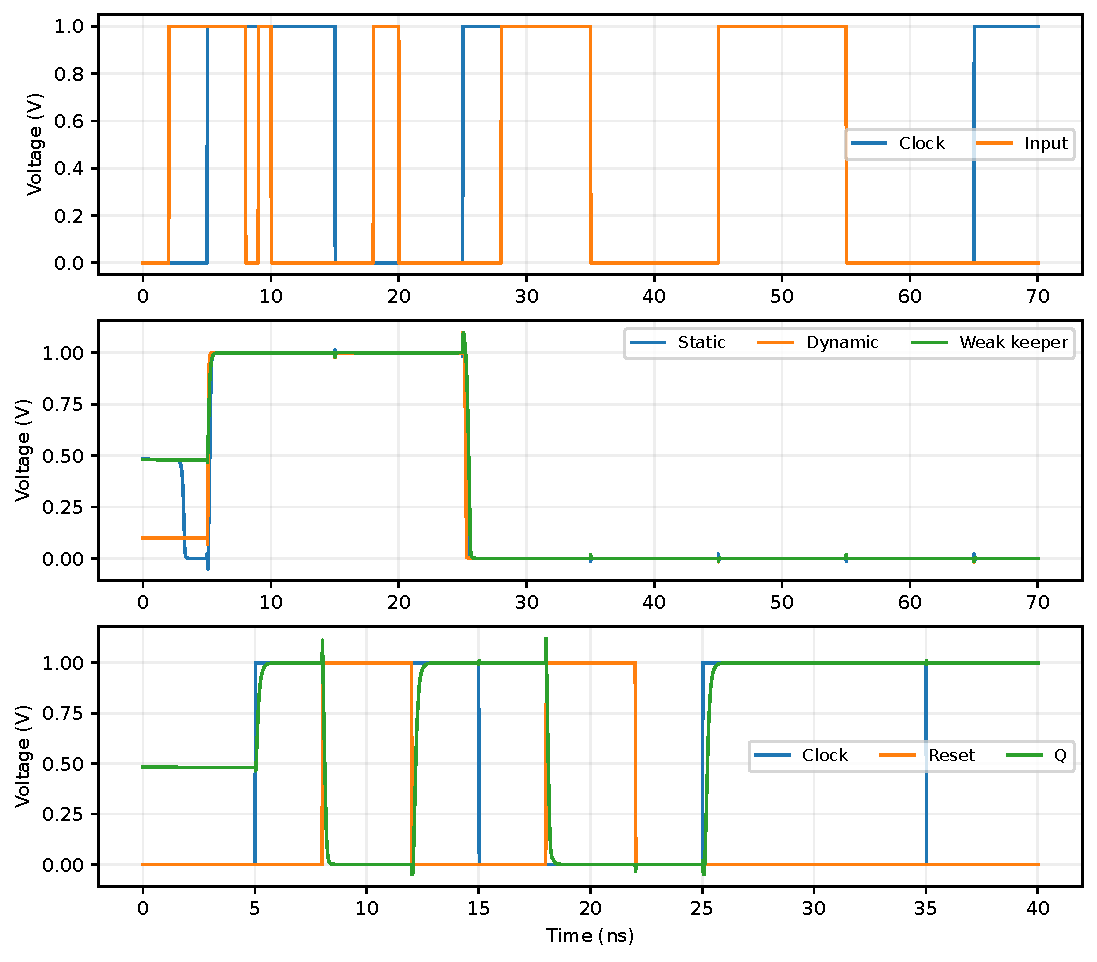
\includegraphics[width=.96\linewidth]{figures/hazards_and_reset.pdf}
\caption{上兩圖為資料 hazard 與三種 DFF 輸出；下圖為兩個時脈相位中的非同步 reset。}
\end{figure}

7、27、47、67 ns 的三組輸出皆約為 1、0、0、0 V。位於關閉相位的資料脈衝未直接傳到輸出；靠近取樣邊緣的 45 ns 轉換刻意落在 setup/hold 邊界，不能由一條波形斷言所有邊緣附近 hazard 都被安全濾除。

\begin{center}
\small
\setlength{\tabcolsep}{4pt}
\begin{tabular}{lrrr}
\toprule
耦合 (fF) & 靜態峰值 (V) & 動態峰值 (V) & 弱回授峰值 (V) \\
\midrule
1 & 0.00263 & 0.01208 & 0.01641 \\
5 & 0.00375 & 0.00814 & 0.01172 \\
20 & 0.06041 & 1.04148 & 0.99972 \\
\bottomrule
\end{tabular}
\end{center}

\begin{figure}[htbp]
\centering
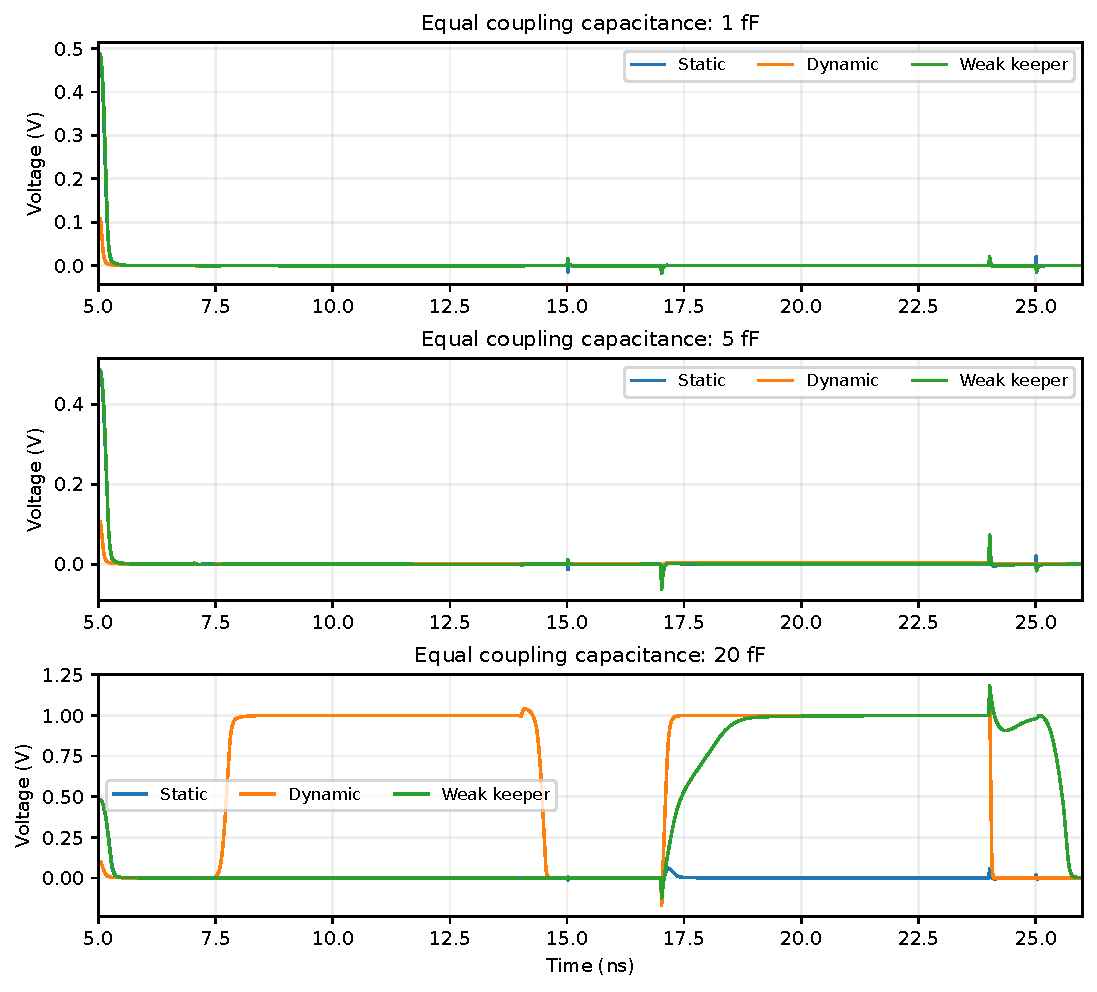
\includegraphics[width=.96\linewidth]{figures/noise.pdf}
\caption{相同電容與 aggressor 分別耦合 master/slave；固定輸入為 0。}
\end{figure}

20 fF 強擾動下靜態輸出峰值僅 0.06041 V，而動態與弱回授約 1.04148 與 0.99972 V，出現錯誤高電位。弱回授改善保持不代表能抵抗任意大擾動；1/5 fF 的小擾動峰值也不必隨電容單調，因為量測含不同注入相位及回復過程。

\subsection{頻率邊界與 reset}

\begin{center}
\small
\setlength{\tabcolsep}{4pt}
\begin{tabular}{lrrr}
\toprule
週期 (ns) & 頻率 (GHz) & 靜態正確/8 & 動態正確/8 \\
\midrule
2 & 0.5000 & 8 & 8 \\
1.8 & 0.5556 & 8 & 8 \\
1.6 & 0.6250 & 8 & 8 \\
1.4 & 0.7143 & 4 & 8 \\
1.2 & 0.8333 & 4 & 8 \\
1 & 1.0000 & 0 & 4 \\
\bottomrule
\end{tabular}
\end{center}

\begin{figure}[htbp]
\centering
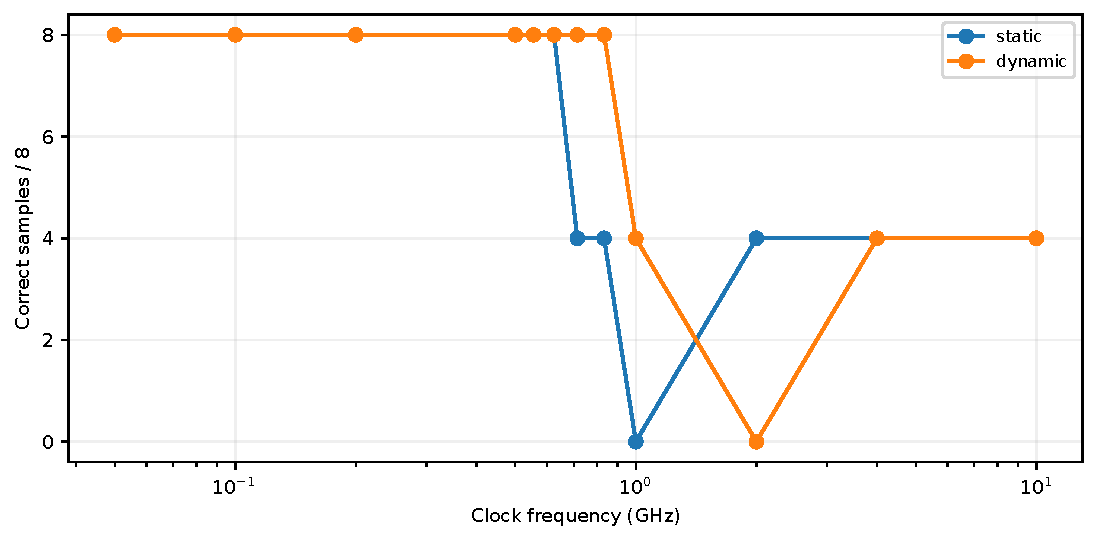
\includegraphics[width=.96\linewidth]{figures/frequency.pdf}
\caption{12 個測試週期的固定時點判讀；連線僅引導視線，不是連續頻率驗證。}
\end{figure}

時脈在 $0.25T$ 開始上升，於每週期 $0.49T$ 取樣，也就是給約 $0.24T$ 的輸出建立時間。最高已測 8/8 正確頻率為靜態 0.625 GHz（1.6 ns）、動態 0.8333 GHz（1.2 ns）；相鄰失敗點分別為 0.7143 GHz（1.4 ns）與 1 GHz。這是特定負載、20 ps 時脈斜率及判讀期限下的有限掃描界線，不能稱為無條件 $f_{\max}$。

reset 在高、低相位的輸出分別為 0.0001976 V 與 $3.395\,\mu$V，解除後重新取樣為 0.999979 V。

\section{討論、差異與尚未證實的範圍}

問題 1：互補時脈若有重疊導通，master/slave 可能同時透明而 race through。問題 2：慢邊緣延長開關半導通與競爭區，也改變可用建立時間；不能只憑名義週期判斷。問題 3：setup 要讓 master 儲存節點在關閉前建立，hold 要避免新資料在關閉完成前穿透；這與時脈轉換斜率、TG 延遲及內部再生相關，並非理想邏輯圖的零時間限制。本報告沒有宣稱已完成連續 setup/hold 或 metastability 萃取；Lab21 另做斜率及 skew 實測。所有比較採相同輸出負載與相同注入擾動，避免把不匹配測試誤稱為抗雜訊優勢。
